\section{E-LQTP Design}
\label{sec:design}

E-LQTP is LQARP plus a dual-track relative-motion estimator, a
persistence-gated HELLO, an optional pair of reward modifiers, and a
stability pre-filter on the candidate set.
The validated operating point uses the estimator and the trigger and
sets the reward modifiers to zero.
Fig.~\ref{fig:mechanism} is the per-tick mechanism;
Algorithm~\ref{alg:elqtp} is the same loop in the equation-referenced
form of LQARP's Algorithm~1 \cite{liu2026lqarp}.
\begin{figure*}[!t]
\centering
\includegraphics[width=\textwidth]{elqtp_figs/fig_mechanism}
\caption{E-LQTP per-tick mechanism.
(a)~Discovery: sensing, dual-track estimation, event trigger, and
rising-edge HELLO.
(b)~Forwarding at $\beta_1=\beta_2=0$, inherited from LQARP.}
\label{fig:mechanism}
\end{figure*}


\subsection{Kinematic State}
\label{sec:design:kin}
For each directed pair $(s_i,s_j)$,
\begin{align}
\label{eq:rel}
p_{ij}(t)&=p_i(t)-p_j(t),\nonumber\\
\dot{p}_{ij}(t)&=\dot{p}_i(t)-\dot{p}_j(t),\nonumber\\
v_{\mathrm{rel}}(i,j)
&= \bigl(\dot{p}_{ij}\cdot p_{ij}\bigr)/\|p_{ij}\|.
\end{align}
Negative $v_{\mathrm{rel}}$ is closing range.
Own velocity $\dot{p}_i$ is odometry and is known exactly.
Neighbor velocity $\dot{p}_j$ is a zero-order hold.
Before any hold has been written the hold is $(0,0,0)$.
Under the shared current of Scenario~II that initialization assigns
pair $(i,j)$ the relative velocity $\dot{p}_i$, which is not the
true relative velocity of two relays drifting together.
The assignment is intentional: writing $j$'s true velocity at
$t=0$ would make every AUV--AUV pair a perfect match to the
constant-velocity model and would leave the trigger with no
innovation on those pairs.
On every later tick for which $\mathrm{Broadcast}_k(i,j)=1$,
including ticks on which the flag stays high after the rising edge,
the three velocity components of the corrected track are overwritten
with no blending,
$\hat{x}_{k|k}^{(v)}\leftarrow\dot{p}_i-\dot{p}_j^{\mathrm{live}}$,
and the forecast track is reset to that corrected state.
The optional drift term does not use the initial hold.
Until the first overwrite, $\beta_2$ is omitted and
$c_{\mathrm{drift}}=c_{\mathrm{del}}$.
SNR does not observe the velocity block.
Horizontal range is adjusted only through the predict Jacobian of
Section~\ref{sec:design:ekf}.
The velocity hold is therefore the sole source of $v_{\mathrm{rel}}$
for the optional drift term.

Scenario~II kinematics are
$\dot{p}_i(t)=v_{\mathrm{drift}}^{(0)}$ with
$\|v_{\mathrm{drift}}^{(0)}\|$ swept in
$[0.5,3.5]\,\mathrm{m/s}$ (reported midpoint $2\,\mathrm{m/s}$)
and one horizontal azimuth, drawn once per run and shared by every relay.
Scenario~III uses a Rankine-capped counterclockwise eddy of core
radius $R_{\mathrm{core}}=2000\,\mathrm{m}$ and speed
$V_{\mathrm{eddy}}=2\,\mathrm{m/s}$ centered at $(3000,3000)\,\mathrm{m}$,
\begin{equation}
\label{eq:rankine}
v_\theta(r)=V_{\mathrm{eddy}}\min(r/R_{\mathrm{core}},1),
\end{equation}
plus the discrete Gauss--Markov step
\begin{equation}
\label{eq:gm}
v^i_{k+1}
= \zeta v^i_k + (1-\zeta)\,v_{\mathrm{eddy}}(p_i)
+ \sqrt{1-\zeta^2}\,\sigma\odot w^i_k,
\end{equation}
with $\zeta=0.95$, $dt=1\,\mathrm{s}$,
$\sigma=(1,1,0)\,\mathrm{m/s}$, and $w^i\sim\mathcal{N}(0,I)$.
The zero vertical innovation is a modelling choice: mid-latitude
mesoscale flow at these scales is geostrophic, and a $1\,\mathrm{m/s}$
vertical term would empty the column.
Inside the solid-body core the mean-flow pair difference is
perpendicular to the line of sight; the Gauss--Markov innovation
supplies most of the observable radial projection
(mean $|v_{\mathrm{radial}}|\approx 1.06\,\mathrm{m/s}$ against
mean $|v_{\mathrm{tangential}}|\approx 2.54\,\mathrm{m/s}$ on the
kinematics-only diagnostic).

\subsection{Dual-Track EKF and Event Trigger}
\label{sec:design:ekf}
\begin{figure*}[!t]
\centering
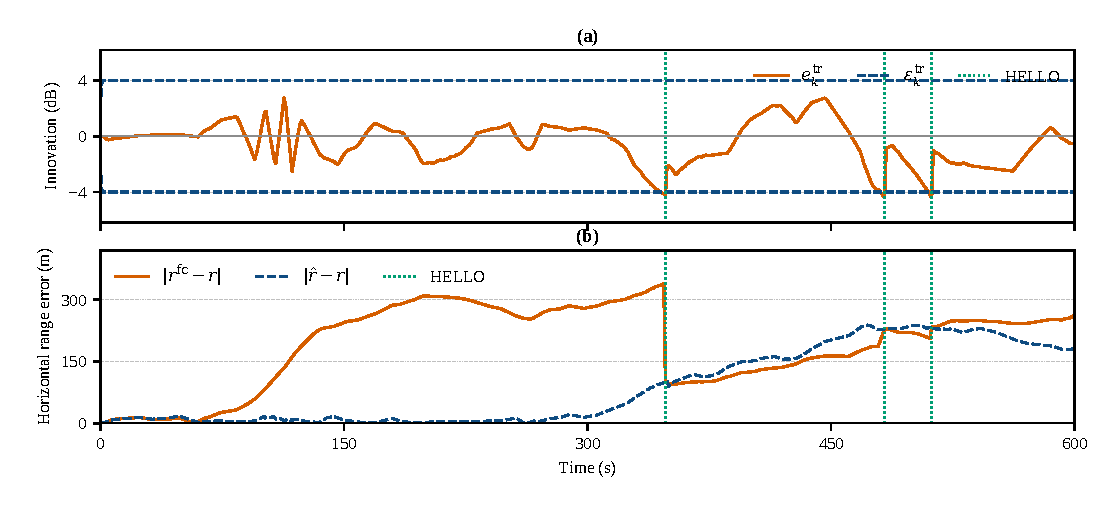
\includegraphics[width=\textwidth]{elqtp_figs/fig7_trigger_trace}
\caption{Dual-track trigger, pair $(1,2)$. (a)~$e_k^{\mathrm{tr}}$
and $\pm\varepsilon_k^{\mathrm{tr}}$. (b)~Range error. HELLOs at
$348$, $483$, $512\,\mathrm{s}$.}
\label{fig:trigger_trace}
\end{figure*}

Each neighbor pair carries a seven-dimensional state
\begin{equation}
\label{eq:state}
x_k=\bigl[p_{ij}^\top,\,\dot{p}_{ij}^\top,\,\mathrm{SNR}_{ij}\bigr]^\top.
\end{equation}
The position--velocity block is constant-velocity,
\begin{equation}
\label{eq:Fkin}
F_{\mathrm{kin}}
=\begin{bmatrix} I_3 & dt\,I_3 \\ 0_3 & I_3 \end{bmatrix},
\end{equation}
and does not carry SNR.
Both tracks apply the same nonlinear predict.
Writing $p^+=p+dt\,\dot{p}$ and
$r_H^+=\|(p_x^+,p_y^+)\|$ for the predicted horizontal range,
with $z_q$ the neighbor's acoustic query depth,
\begin{equation}
\label{eq:forecast}
\begin{aligned}
p^+&=p+dt\,\dot{p},&
\dot{p}^+&=\dot{p},\\
\mathrm{SNR}^+
&=
\begin{cases}
\mathrm{SNR}(r_H^+,z_q), & \text{if the lookup is finite},\\
\mathrm{SNR}^-, & \text{otherwise,}
\end{cases}
\end{aligned}
\end{equation}
The lookup is \eqref{eq:snr}.
An out-of-envelope cell keeps the last finite SNR; it is not
interpolated.
The covariance is propagated by the $7\times 7$ Jacobian $F$ of
\eqref{eq:forecast}: $F=I_7$, the three constant-velocity couplings
are $F_{1,4}=F_{2,5}=F_{3,6}=dt$, the SNR row is replaced rather
than scaled so $F_{7,7}=0$, and the only nonzero SNR--position
entries are the horizontal radial derivatives
\begin{equation*}
F_{7,1}
=\frac{\partial\mathrm{SNR}}{\partial r_H}\frac{p_x^+}{r_H^+},\qquad
F_{7,2}
=\frac{\partial\mathrm{SNR}}{\partial r_H}\frac{p_y^+}{r_H^+}.
\end{equation*}
The range derivative is a central difference with step
$10\,\mathrm{m}$.
Process noise is then added on the diagonal,
$P^+=FPF^\top+Q$, with
$q_{\mathrm{pos}}=1.0$, $q_{\mathrm{vel}}=0.1$, and
$q_{\mathrm{SNR}}=1.0$.
The measurement variance is
$R=r_{\mathrm{meas}}=4.0\,\mathrm{dB}^2$.

Two tracks run in parallel and share \eqref{eq:forecast}.
The \emph{corrected} track $(\hat{x},P)$ also applies a measurement
update.
The raw sample $z_k$ is the Bellhop SNR at the nodes' true current
positions, computed every $dt$ whether or not a packet is heard.
The median $\tilde{z}_k$ is taken over the samples stored for that
pair, at most $W_{\mathrm{mp}}=3$; the first ticks use the shorter
prefix.
The one-step innovation
$e_k=\tilde{z}_k-\hat{x}^{\mathrm{SNR}}_{k|k-1}$
enters the filter and, optionally, $c_{\mathrm{pred}}$.
The update uses $H=[0\,0\,0\,0\,0\,0\,1]$ because the measurement
is the SNR component.
The gain is the corresponding column of $P$,
$K=P_{:,7}/S_k$ with $S_k=P_{7,7}+r_{\mathrm{meas}}$, so the
innovation moves every state component that has covariance with SNR.
Horizontal range is among those components because $F_{7,1}$ and
$F_{7,2}$ couple predicted range into the SNR variance.
The tangential directions and the velocity block are not directly
observed by $H$.
The \emph{forecast} track $(x^{\mathrm{fc}},P^{\mathrm{fc}})$
receives the predict and no measurement update.
It is reset to $(\hat{x}_{k|k},P_{k|k})$ on every tick with
$\mathrm{Broadcast}_k(i,j)=1$, after the corrected-track update,
by the velocity overwrite of Section~\ref{sec:design:kin}.
The trigger innovation uses the raw query against the forecast SNR,
which \eqref{eq:forecast} has just set to the lookup at the
forecast range,
\begin{equation}
\label{eq:etrigger}
e_k^{\mathrm{tr}}
= z_k - \mathrm{SNR}\bigl(r_H(x^{\mathrm{fc}}_k),z_q\bigr).
\end{equation}
A one-step $e_k$ cannot form this residual: the corrected track is
healed every tick, whereas $x^{\mathrm{fc}}$ accumulates the motion
implied by the held velocity.

The corrected-track threshold is left uncapped.
The forecast covariance is not measurement-updated, so
$\varepsilon_0+\lambda\sqrt{S_k^{\mathrm{tr}}}$ would make a
long-silent pair progressively harder to trigger.
The trigger threshold therefore caps the uncertainty term,
\begin{equation}
\label{eq:eps}
\begin{aligned}
\varepsilon_k
&= \varepsilon_0+\lambda\sqrt{S_k},\\
\varepsilon_k^{\mathrm{tr}}
&= \varepsilon_0+\lambda\min\bigl(\sqrt{S_k^{\mathrm{tr}}},
s_{\mathrm{cap}}\bigr),
\end{aligned}
\end{equation}
with $\varepsilon_0=2.0\,\mathrm{dB}$, $\lambda=1$,
$s_{\mathrm{cap}}=\sqrt{r_{\mathrm{meas}}}=2.0\,\mathrm{dB}$,
$S_k=P_{7,7}+r_{\mathrm{meas}}$, and
$S_k^{\mathrm{tr}}=P^{\mathrm{fc}}_{7,7}+r_{\mathrm{meas}}$.
The cap is the design choice identified in
Section~\ref{sec:intro}; it is not taken from
\cite{busacca2024snr}.
A persistence gate with width $W=5$ and fraction $\rho=0.6$ then
sets the flag.
Let $n_k$ be the number of finite trigger samples retained for the
pair, at most $W$.
Until five samples have been stored, $n_k$ is that shorter prefix,
so a single early exceedance has fraction one and can pass
$\rho$.
\begin{equation}
\label{eq:bc}
\begin{aligned}
\mathrm{Broadcast}_k&=1
\quad\text{if }|e_k^{\mathrm{tr}}|\ge\varepsilon_k^{\mathrm{tr}}\\
&\quad\text{and }
\tfrac{1}{n_k}\textstyle\sum_{m\in\mathcal{W}_k}
\mathbf{1}\{|e_m^{\mathrm{tr}}|\ge\varepsilon_m^{\mathrm{tr}}\}\ge\rho,\\
\mathrm{Broadcast}_k&=0
\quad\text{otherwise,}
\end{aligned}
\end{equation}
where $\mathcal{W}_k$ is the retained window.
A non-finite $z_k$ skips the update and forces
$\mathrm{Broadcast}_k=0$.
Node $j$ originates one HELLO on a tick if
$\mathrm{Broadcast}_k(i,j)$ rises for any observer $i$.
Ticks on which the flag merely stays high do not add a further
transmission.
Those ticks do repeat the velocity overwrite and the forecast reset.

Fig.~\ref{fig:trigger_trace} shows the two tracks on
Scenario~III pair $(1,2)$.
Panel~(a) is $e_k^{\mathrm{tr}}$ against
$\pm\varepsilon_k^{\mathrm{tr}}$; the threshold sits at the
$s_{\mathrm{cap}}$ ceiling once forecast variance has grown.
Rising-edge HELLOs occur at $t=348$, $483$, and $512\,\mathrm{s}$.
Panel~(b) is the corresponding horizontal range error.
The forecast range error grows while the flag is low and is reset
when the flag is high.
The corrected range error stays smaller because the per-tick query,
acting through $K$, heals the radial state.
That is the mechanism the control-plane results of
Section~\ref{sec:eval} attribute the overhead reduction to.

\begin{algorithm}[!t]
\caption{E-LQTP: Event-Triggered HELLO and Q-Learning Forwarding}
\label{alg:elqtp}
\begin{algorithmic}[1]
\REQUIRE poses $(p_i,\dot{p}_i)$; hold $\dot{p}_j\leftarrow 0$ until written;
$(\hat{x},P)$, $(x^{\mathrm{fc}},P^{\mathrm{fc}})$
\ENSURE one HELLO per rising node; $s_i.\mathrm{NextHop}$
\STATE {\bfseries Discovery:} dual-track predict \eqref{eq:forecast}
\FOR{each directed pair $(i,j)$}
  \STATE Predict both tracks by \eqref{eq:forecast}, using \eqref{eq:Fkin}
  \STATE $z_k\leftarrow\mathrm{SNR}(p_i,p_j)$ \eqref{eq:snr}
        \COMMENT{\cite{liu2026lqarp}}
  \IF{$z_k$ is non-finite}
    \STATE skip update; $\mathrm{Broadcast}_k(i,j)\leftarrow 0$
  \ELSE
    \STATE $\tilde{z}_k\leftarrow$ median of the stored prefix, at most $W_{\mathrm{mp}}$
    \STATE $e_k\leftarrow\tilde{z}_k-\hat{x}^{\mathrm{SNR}}$;
          $e_k^{\mathrm{tr}}$ from \eqref{eq:etrigger}
    \STATE $\varepsilon_k$ and $\varepsilon_k^{\mathrm{tr}}$ from \eqref{eq:eps}
    \STATE EKF-update $(\hat{x},P)$ on $\tilde{z}_k$ with $H=[0\,\cdots\,1]$
    \STATE $\mathrm{Broadcast}_k(i,j)$ from \eqref{eq:bc}
    \IF{$\mathrm{Broadcast}_k(i,j)=1$}
      \STATE $\hat{x}^{(v)}\leftarrow\dot{p}_i-\dot{p}_j^{\mathrm{live}}$;
            reset forecast to $(\hat{x},P)$
    \ENDIF
  \ENDIF
\ENDFOR
\IF{event-triggered}
  \STATE node $j$ sends one HELLO if any $i$ has a $0\to 1$ edge on $(i,j)$
\ELSIF{Fixed-Periodic \textbf{and} $t\bmod T_{\mathrm{ctrl}}=0$}
  \STATE every node sends one HELLO; every pair ingests $\dot{p}_j^{\mathrm{live}}$
\ENDIF
\STATE {\bfseries Forwarding:} LQARP Q-learning
      \cite{liu2026lqarp}
\IF{node $s_i$ has a data packet}
  \STATE $I_{\mathrm{ELQTP}}$ from \eqref{eq:cand}, \eqref{eq:nstab};
        detour if empty \COMMENT{\cite{liu2026lqarp}}
  \STATE reward \eqref{eq:reward_elqtp}; TD update \eqref{eq:q}
        \COMMENT{\cite{nandyala2023qtar}}
  \STATE $s_i.\mathrm{NextHop}\leftarrow\arg\max Q$
\ENDIF
\end{algorithmic}
\end{algorithm}

\subsection{Reward Terms}
\label{sec:design:reward}
E-LQTP replaces $c_{\mathrm{lin}}$ and $c_{\mathrm{del}}$ with
\begin{align}
\label{eq:cpred}
c_{\mathrm{pred}}
&= c_{\mathrm{lin}}
+\beta_1\max\bigl(0,e_k-e_{k-1}\bigr),\\
\label{eq:cdrift}
c_{\mathrm{drift}}
&= c_{\mathrm{del}}
\bigl(1+\beta_2\,\sigma(-v_{\mathrm{rel}})\bigr),
\end{align}
where $\sigma(u)=(1+e^{-u})^{-1}$.
If $i$ has not yet heard $j$, the $\beta_2$ factor is omitted
($c_{\mathrm{drift}}=c_{\mathrm{del}}$).
The composite reward is
\begin{equation}
\label{eq:reward_elqtp}
R^{a_j}_{s_i,s_j}
= \frac{c_{\mathrm{ene}}(s_j)\,c_{\mathrm{drift}}(s_i,s_j)\,
c_{\mathrm{nei}}(s_j)}{c_{\mathrm{pred}}(s_i,s_j)}.
\end{equation}
$\beta_1=\beta_2=0$ recovers \eqref{eq:reward_lqarp} exactly and is
the validated default.
The Q-update is \eqref{eq:q} over the restricted action set of
Section~\ref{sec:design:cand}.

The additive form \eqref{eq:cpred} is scale-inconsistent on the
BER-floor plateau: a typical one-step $\Delta e_k$ is
$\mathcal{O}(0.01)\,\mathrm{dB}$, so an $\mathcal{O}(1)$ $\beta_1$
overrides $c_{\mathrm{lin}}\approx 4\times 10^{-7}$ by four orders
of magnitude.
A blend-scale $\beta_1$ ($10^{-5}$--$10^{-6}$) has no favorable
effect either (Section~\ref{sec:eval:beta}).
The one-step Kalman trend persists for only about one second
(median same-sign run $1$--$4\,\mathrm{s}$, $25$th percentile
$1\,\mathrm{s}$), comparable to or shorter than a hop
($\approx 2\,\mathrm{s}$).
$c_{\mathrm{drift}}$ has no scale bug, but under the eddy the
radial-velocity sign persists for a median $3\,\mathrm{s}$
($25$th percentile $1\,\mathrm{s}$), so the
persistent-closing-range assumption does not hold.
Both findings are scoped negative results.

\subsection{Candidate Set}
\label{sec:design:cand}
E-LQTP adds a fourth filter to \eqref{eq:cand},
\begin{equation}
\label{eq:nstab}
\begin{aligned}
N_{\mathrm{stab}}(s_i)
&=\bigl\{s_j:\mathrm{Broadcast}_k(i,j)=0\bigr\}\\
&\quad\cup
\bigl\{s_j:|e_k(i,j)|<\varepsilon_k(i,j)\bigr\},
\end{aligned}
\end{equation}
and forwards on
$I_{\mathrm{ELQTP}}(s_i)
=N_{\mathrm{range}}\cap N_{\mathrm{SNR}}\cap N_{\mathrm{depth}}
\cap N_{\mathrm{stab}}$.
Here $e_k$ and $\varepsilon_k$ are the corrected-track innovation and
the uncapped threshold in \eqref{eq:eps}, not
$(e_k^{\mathrm{tr}},\varepsilon_k^{\mathrm{tr}})$.
The leftover $0.2\%$ hop difference versus LQARP on Scenario~III
is this pre-filter with the trigger on, not a reward term.
The detour of Section~\ref{sec:prelim:q} is unchanged.

\subsection{Packets and Control Accounting}
\label{sec:design:pkt}
A data packet is $l=400\,\mathrm{bit}$ at $R_b=1000\,\mathrm{bit/s}$
(airtime $0.4\,\mathrm{s}$) and carries the payload plus a
visited-node list for detour loop prevention (TTL $32$).
A dedicated HELLO is charged at the same $400\,\mathrm{bit}$.
Its timing, the single transmission by node $j$, and the oracle
velocity copy are those of Section~\ref{sec:design:ekf}: the payload
is not demodulated, and the copy is written only into the velocity
hold.
Forwarding for every protocol reads the simulator's current pose,
residual energy, and a fresh Bellhop sample at the decision
instant, as stated in Section~\ref{sec:prelim:est}.
LQARP and the RLOR-inspired baseline generate no dedicated control
frames, so their $O_{\mathrm{ctrl}}$ is identically zero.
E-LQTP and Fixed-Periodic add HELLO bytes on top of that shared
data plane.
HELLO joules enter $O_{\mathrm{ctrl}}$ only.
A control transmission leaves residual energy and data-packet
reception unchanged.
Control overhead is
\begin{equation}
\label{eq:octrl}
O_{\mathrm{ctrl}}
= \frac{\text{control bytes on }[0,T_{\mathrm{sim}}]}{T_{\mathrm{sim}}}.
\end{equation}
Drain-period control traffic is not billed.
Fixed-Periodic replaces \eqref{eq:bc} with the grid
$t=0,T_{\mathrm{ctrl}},2T_{\mathrm{ctrl}},\ldots$ at
$T_{\mathrm{ctrl}}=5\,\mathrm{s}$ and is otherwise identical, so
the ablation isolates timing.

\subsection{Simulation Implementation}
\label{sec:design:ns3}
The protocols are implemented in ns-3.41 with Aqua-Sim-NG and share
one Bellhop lookup path \cite{liu2026lqarp}.
Scenario~I holds every node fixed; Scenarios~II and~III use
constant-velocity kinematics with poses read at every forwarding
event and every EKF tick.
The same random placement is used for all four protocols.
Reception is an SNR-threshold test on the shared Bellhop sample.
Collisions, backoff, and idle listening are omitted, so control
airtime does not delay or drop a data packet.
The RLOR-inspired baseline follows the brief sketch in
\cite{liu2026lqarp} and the opportunistic class surveyed in
\cite{jiang2023orsurvey}.
That sketch does not specify a line-by-line algorithm, so the
baseline used here takes the candidate set
$N_{\mathrm{range}}\cap N_{\mathrm{SNR}}$ (no $N_{\mathrm{depth}}$,
no detour) and forwards
$\arg\max P_{\mathrm{succ}}$ with no Q-table.
\FloatBarrier
